\documentclass[xcolor=x11names,compress,professionalfonts]{beamer}

%% General packages %%%%%%%%%%%%%%%%%%%%%%%%%%%%%%%%%%
\usepackage[utf8]{inputenc}
\usepackage{graphicx}
\usepackage{tikz}
\tikzset{% change default arrow tips
    >=latex
}
\usepackage{ifthen}

\usepackage{amsmath}
\usepackage{nicefrac}

\usepackage{color}

%%%%%%%%%%%%%%%%%%%%%%%%%%%%%%%%%%%%%%%%%%%%%%%%%%%%%%


%% Beamer Layout %%%%%%%%%%%%%%%%%%%%%%%%%%%%%%%%%%
\useoutertheme[subsection=false,shadow]{miniframes}
\useinnertheme{rectangles}

\setbeamertemplate{navigation symbols}{}%remove navigation symbols

\newcommand{\btVFill}{\vskip0pt plus 1filll}%place an element at the bottom of the page

\usepackage{libertine}
\usepackage[T1]{fontenc}

\setbeamerfont{title like}{shape=\scshape}
\setbeamerfont{frametitle}{shape=\scshape}

\setbeamercolor*{lower separation line head}{bg=DeepSkyBlue4} 
\setbeamercolor*{normal text}{fg=black,bg=white} 
\setbeamercolor*{alerted text}{fg=red} 
\setbeamercolor*{example text}{fg=black} 
\setbeamercolor*{structure}{fg=black} 
 
\setbeamercolor*{palette tertiary}{fg=black,bg=black!10} 
\setbeamercolor*{palette quaternary}{fg=black,bg=black!10} 

\renewcommand{\(}{\begin{columns}}
\renewcommand{\)}{\end{columns}}
\newcommand{\<}[1]{\begin{column}{#1}}
\renewcommand{\>}{\end{column}}

\definecolor{BostonBlue}{HTML}{00688B}
\definecolor{Complementary}{HTML}{8B2300}
%%%%%%%%%%%%%%%%%%%%%%%%%%%%%%%%%%%%%%%%%%%%%%%%%%

\usepackage{braket}
% compile child documents using this preamble
\usepackage{subfiles}

%%%My Math

\newcommand{\pd}[2]{\frac{\displaystyle \partial #1}{\displaystyle\partial #2}} % for partial derivatives
\newcommand{\dx}{\mathrm{d}x}
\renewcommand{\d}[1]{\mathrm{d}#1}
\newcommand{\nth}{$n^\text{th}$ }

\newcommand{\mean}[1]{\langle #1 \rangle}
\DeclareMathOperator{\Pf}{Pf}
\DeclareMathOperator{\Tr}{Tr}

% idos
\newcommand{\id}{\ensuremath{\text{idos}}}
% mean energy of a gap
\newcommand{\me}{\ensuremath{\langle E \rangle}}
\newcommand{\mep}{\ensuremath{\langle E' \rangle}}
% bold g letter in math mode
\newcommand{\gv}{\ensuremath{\mathbf{g}}}
% the symbol used for the Fibonacci substitution matrix
\newcommand{\sub}{\ensuremath{M}}
% letters A and B appearing in the qp chains
\newcommand{\A}{\textcolor{BostonBlue}{A}}
\newcommand{\B}{\textcolor{Complementary}{B}}

\begin{document}


\begin{frame}
\title{{\fontsize{14}{60}\selectfont Gap structure of 1D cut and project Hamiltonians}}

\author{Nicolas Macé, Anuradha Jagannathan, Frédéric Piéchon \\ special thanks to Jean-Noël Fuchs}

\institute % (optional)
{
  Laboratoire de Physique des Solides\\
  Université Paris-Saclay
}

\date{September 20, 2016}

\titlepage

\btVFill
\begin{columns}
\begin{column}{2cm}
~\\
~\\
~\\
~\\
\raggedright

\includegraphics[scale=.15]{img/LogoUPSUD.png}
\end{column}
\begin{column}{6cm}
\centering
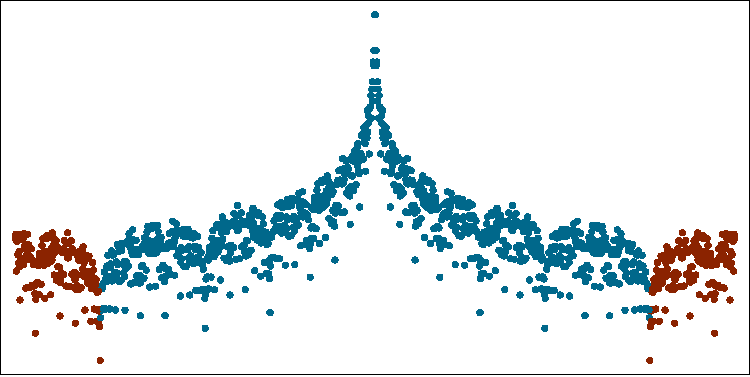
\includegraphics[width=1.\textwidth]{img/cover_illustration.pdf}
\end{column}
\begin{column}{2cm}
~\\
~\\
~\\
~\\
\raggedleft

\includegraphics[scale=.15]{img/logo-lps.jpg}
\end{column}
\end{columns}
\end{frame}

\begin{frame}
\frametitle{Outline}
\tableofcontents[hideallsubsections]
\end{frame}

\section{The gap labeling theorem}
%Each section needs a subsection for the small points on top to show up
\subsection{Dummy}

\begin{frame}{Electrons on quasiperiodic chains}

Canonical cut and project method of slope $\alpha$ $\rightarrow$ chain of two letters:

{\centering
\dots\A\B\A\A\B\A\B\A\A\B\A\A\B\A\B\A\A\B\A\B\A\dots

}

Quantum model:

{\centering
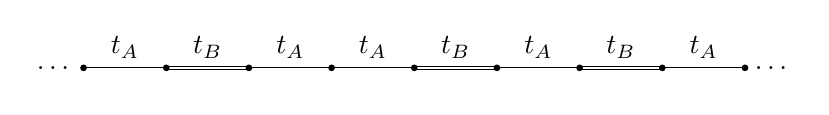
\begin{tikzpicture}[scale=.7]
    		\newcommand{\orig}{-1.5}
    		\newcommand{\trans}{1.5}
    		\newcommand{\vertspac}{-2.}
    	
    		% initial chain
    	
    		% bonds 
        	\draw[-] (\orig+\trans,0) -- (\orig+2*\trans,0) node [midway, above] {$t_A$};
			\draw[-,double] (\orig+2*\trans,0) -- (\orig+3*\trans,0) node [midway, above] {$t_B$};	
			\draw[-] (\orig+3*\trans,0) -- (\orig+4*\trans,0) node [midway, above] {$t_A$};
			\draw[-] (\orig+4*\trans,0) -- (\orig+5*\trans,0) node [midway, above] {$t_A$};
			\draw[-,double] (\orig+5*\trans,0) -- (\orig+6*\trans,0) node [midway, above] {$t_B$};
			\draw[-] (\orig+6*\trans,0) -- (\orig+7*\trans,0) node [midway, above] {$t_A$};
			\draw[-,double] (\orig+7*\trans,0) -- (\orig+8*\trans,0) node [midway, above] {$t_B$};
			\draw[-] (\orig+8*\trans,0) -- (\orig+9*\trans,0) node [midway, above] {$t_A$};
    	
    	
    		% sites
		    \filldraw (\orig+1*\trans,0) circle (0.05) node [left] {\dots};
		    \filldraw (\orig+2*\trans,0) circle (0.05) node [below] {};
		    \filldraw (\orig+3*\trans,0) circle (0.05) node [below] {};
		    \filldraw (\orig+4*\trans,0) circle (0.05) node [below] {};
		    \filldraw (\orig+5*\trans,0) circle (0.05) node [below] {};
		    \filldraw (\orig+6*\trans,0) circle (0.05) node [below] {};
		    \filldraw (\orig+7*\trans,0) circle (0.05) node [below] {};
		    \filldraw (\orig+8*\trans,0) circle (0.05) node [right] {};
		    \filldraw (\orig+9*\trans,0) circle (0.05) node [right] {\dots};
		      
\end{tikzpicture}

}

Hamiltonian:  
$ H(\alpha)  = \sum_{x \in \mathbb{Z}} t_{x,x+1} \ket{x} \bra{x+1} + \text{h.c.} $ \\where $t_{x,x+1}  = t_A \text{~or~} t_B$ {\scriptsize(see [Kohmoto 86])}

$t_A/t_B$ is the only parameter of the model.
\(
\<{5cm}
\flushright
Experimental realization with cavity polaritons

{\scriptsize[Tanese \textit{et al} 2015]}
\>

\<{7cm}
\centering
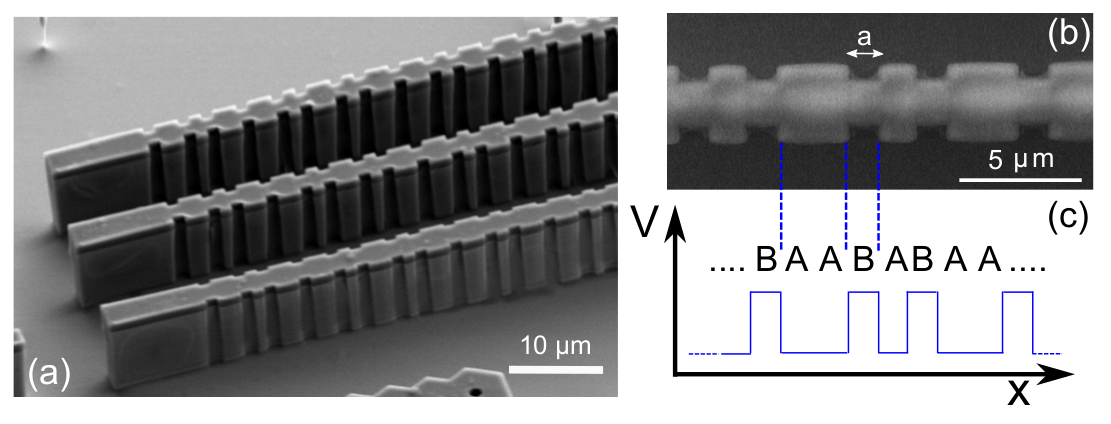
\includegraphics[scale=.15]{img/tanese.png}
\>
\)

\begin{align*}
	\alpha = \frac{m}{n} \in \mathbb{Q} &\implies \text{periodic chain of period } L = m + n \\
	\alpha \in \mathbb{R} \smallsetminus \mathbb{Q} &\implies \text{quasiperiodic chain}
\end{align*}

\end{frame}

\begin{frame}{The energy spectrum}
Well understood: electrons on \emph{periodic} chains (Bloch's theory)

Idea: approach a QP chain $\alpha$ by a sequence of periodic \emph{approximants}:
\[
	\alpha_l = \frac{m_l}{n_l} \xrightarrow[l \to \infty]{} \alpha
\]
$\rightarrow$ energy spectrum consists of $m_l + n_l$ \emph{energy bands}

Fibonacci chain: $\alpha_l = F_{l}/F_{l+1} \xrightarrow[l \to \infty]{} \tau^{-1} = 0.618\dots$

{\centering
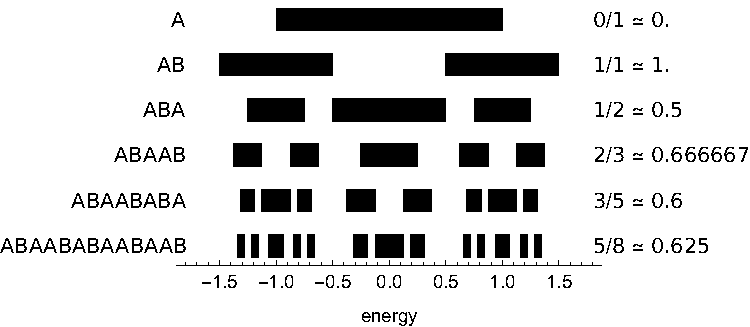
\includegraphics[scale=.8]{img/energy_bands.pdf}

}

\end{frame}

\begin{frame}{\id~ and gap labeling}

A convenient way to plot the spectrum: the integrated density of states ($\id$).

$\id(E) = $ fraction of states below energy $E$

{\centering
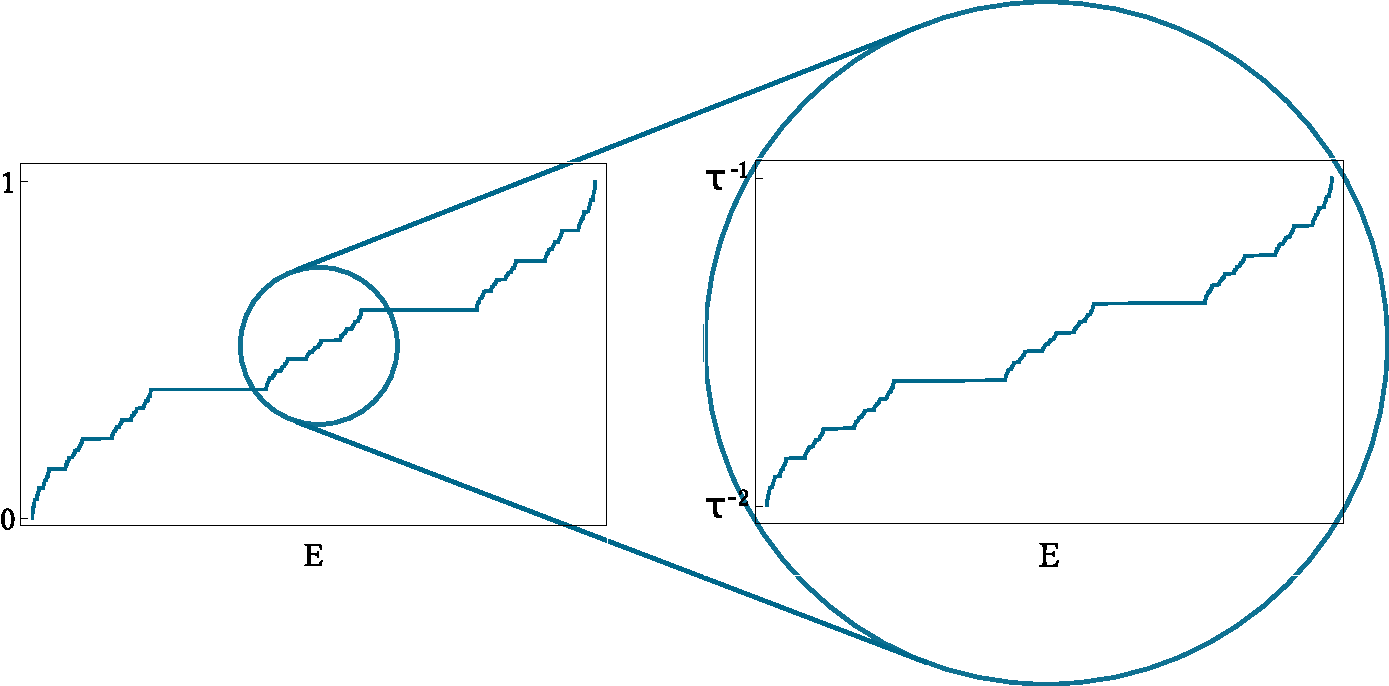
\includegraphics[scale=.35]{img/idos_scaling.pdf}

\small{\id~of the Fibonacci Hamiltonian (devil's staircase)}

}

\begin{itemize}
	\item Electronic spectrum of quasiperiodic chains is hard to describe
	\item Rather: set of $\id$ values in the gaps $\to$ \textbf{gap labeling theorem}
\end{itemize}
\[
	\id(E\in \text{gap}) = p+ q \tau^{-2} 
\]

\end{frame}

\begin{frame}{The gap labeling theorem}
The IDOS inside spectral gaps can be written
	\begin{align*}
		\id(E \in \text{gap}) &= p+\frac{q}{1+\alpha} \\
		\id(E \in \text{gap}) &=  \frac{q}{1+\alpha} \mod 1
	\end{align*}
	where $p, q \in \mathbb{Z}$ are the \emph{gap labels} {\scriptsize see [Bellisard 89]}.
\begin{itemize}
	\item The set of labels constrains the spectrum... but is not enough to reconstruct it
	\item The labels are model independent! 
	\begin{itemize}
		\item In particular, independent of $t_A$ and $t_B$
		\item Gap labels are topological invariants
	\end{itemize}
\end{itemize}

%TODO: plot the idos for the diagonal and the on-site potential models

\end{frame}

\begin{frame}{The gap labeling theorem}
\[
		\id(E \in \text{gap}) = \frac{q}{1+\alpha} \mod 1
\]
\begin{itemize}
	\item Has the gap label $q$ a physical interpretation?
	\item Can the theorem be applied to approximants? 
	\item Does it help understanding the quasiperiodic limit?
\end{itemize}

\end{frame}

\begin{frame}{Gap labeling from Bloch's theory}
Let $\alpha_l = \frac{m_l}{n_l} \to \alpha$ be a sequence of approximants.

Bloch's theorem: there are $L_l = m_l + n_l$ energy bands.

\[
	\id(E \in \text{gap}) = \frac{j(E)}{L_l}
\]
We can find integers $p$, $q$ such that $j = p L_l + q n_l$.
\[
	\id(E \in \text{gap}) = \frac{q n_l}{m_l + n_l} \mod 1
\]
\[
	\id(E \in \text{gap}) = \frac{q }{1+\alpha_l} \mod 1
\]
Letting $l \to \infty$,
	\[
		\id(E \in \text{gap}) = \frac{q}{1+\alpha} \mod 1
	\]

\only<1>{
\phantom{aaa}
}
    
\only<2>{
	\begin{alertblock}{Problem:}
At fixed $j$, $q$ depends on $l$.
\end{alertblock}
}

\end{frame}

\section{The Fibonacci chain}
\subsection{Dummy}

\begin{frame}{Transient and stable gaps}
Gaps of successive approximants of the Fibonacci chain.

{\centering
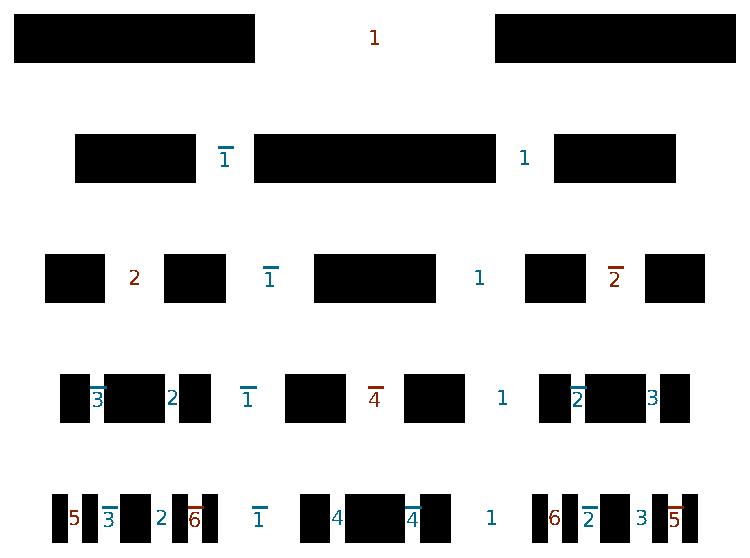
\includegraphics[scale=.8]{img/gap_labels.pdf}

}
\only<1>{
$\me_l$: mean energy of a gap, $\Delta_l(\me)$: its width. 
 
 Identify two gaps if they overlap:
\[
	0.5 \Delta_l(\me) > |\me_l - \mep_{l+1}|
\]
}

\only<2>{
\begin{itemize}
	\item {\color{BostonBlue}Stable gaps} have a fixed label, that does not depend on $l$.
	\item {\color{Complementary}Transient gaps} have a label that is $l$-dependent.
\end{itemize}
}

%\only<3>{
%\begin{itemize}
%	\item {\color{Complementary}Transient} gaps closes as $l \to \infty$
%	\item {\color{BostonBlue}Stable} gaps stay open.
%\end{itemize}
%}
%
%\only<4>{
%\begin{itemize}
%	\item {\color{BostonBlue}Stable gaps:} $n$ independent of $l$ $\rightarrow$ naive proof works.
%	\item {\color{Complementary}Transient gaps:} $n$ depends on $l$, but these gaps disappear.
%\end{itemize}
%$\to$ the naive proof works and correctly labels the gaps.
%}
\end{frame}

\begin{frame}{Examples of transient and stable gaps}

\(
\<{6cm}
\begin{itemize}
	\item The $E=0$ gap 
	\begin{itemize}
		\item is transient
		\item has the label \[q_l = \Big\lfloor \frac{(2+\sqrt{5})^{l/3}}{2 \sqrt{5}} + \frac{1}{2} \Big\rfloor\]
		\item has  vanishing width in the quasiperiodic limit. \\
					\textbf{True for all transient gaps}
	\end{itemize}
	\item The two largest gaps 
	\begin{itemize}
		\item are stable
		\item have label $q = \pm 1$
		\item have a nonzero width in the quasiperiodic limit\\
					\textbf{True for all stable gaps}
	\end{itemize}
\end{itemize}
\>

\<{6cm}
\centering
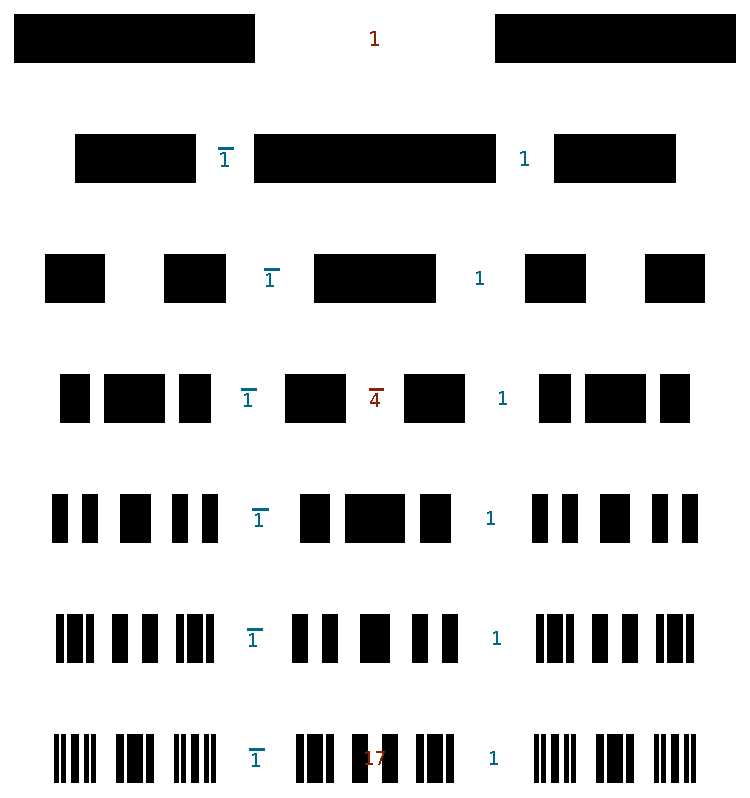
\includegraphics[scale=.45]{img/main_gap_labels.pdf}
\>
\)

\end{frame}

\begin{frame}{Recursive gap labeling}

\begin{columns}
\newcommand{\s}{.2}

  \begin{column}{5cm}
  \centering
     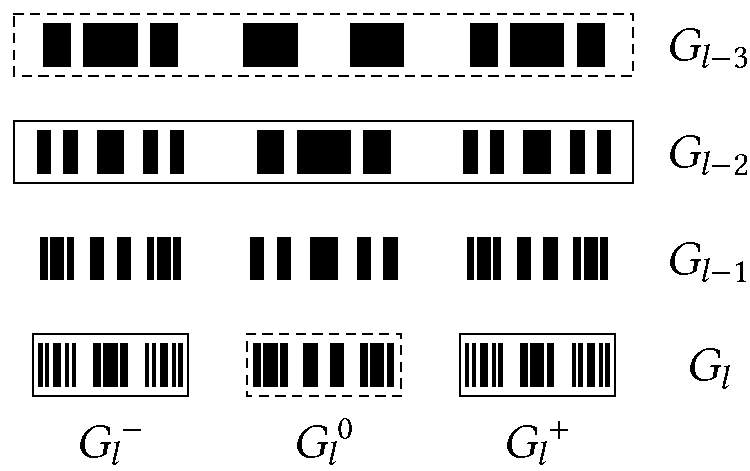
\includegraphics[scale=.4]{img/recursive_construction_spectrum.pdf}
     
	\small{Recursive construction of the spectrum {\scriptsize [Niu, Nori 86]}}
	
  \end{column}


  \begin{column}{5cm}
Let $G_l$ be the set of gap labels:

$\small{G_l = \{(p,q)| \id = p+q/(1+\alpha)\}}$
$G_l$ obeys the recursive relation:
		\begin{align*}
			G_{l}^{-} &= \sub^{-2} G_{l-2} \\
			G_{l}^0 &= \sub^{-3} G_{l-3} + (1, -1) \\
			G_{l}^+ &= \sub^{-2} G_{l-2} + (0,1)
		\end{align*}
$M$ is the \emph{inflation matrix}:
\[
			\sub = \begin{bmatrix}
				1 & 1\\
				1 & 0\\
			\end{bmatrix}
			\rightarrow
			M
			\begin{pmatrix}
			A \\
			B
			\end{pmatrix}
			=
			\begin{pmatrix}
			AB \\
			A
			\end{pmatrix}
			\]
			
  \end{column}
\end{columns}

\begin{itemize}
	\item Geometrical interpretation of the Fibonacci gap labeling
	\item Stable and transient gap are completely characterized:
	\begin{itemize}
		\item {\color{BostonBlue}Stable gaps} are the iterates of the 2 largest gaps
		\item {\color{Complementary}Transient gaps} are the iterates of the $E=0$ gap.
	\end{itemize}	 
\end{itemize}

\end{frame}

\section{General case}
\subsection{Dummy}
\begin{frame}{General case}
\begin{itemize}
	\item We can still distinguish (numerically) stable and transient gaps for various C\&P chains.
$\rightarrow$ the naive argument seem to work.
	\item We plot the gapwidth $\Delta_l$ as a function of the label:
\end{itemize}

\(
\<{6cm}
{\centering
\newcommand{\s}{.45}
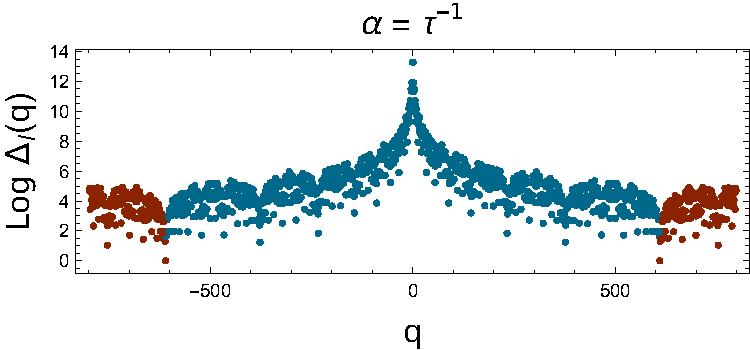
\includegraphics[scale=\s]{img/loggapwidth_fibonacci_l_17.pdf}\\
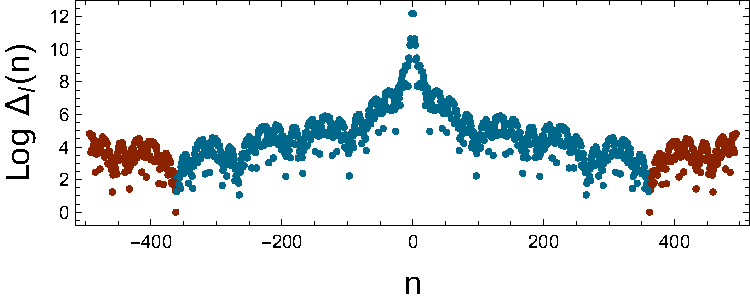
\includegraphics[scale=\s]{img/loggapwidth_sqrt3_l_12.pdf}

}
\>
\<{6cm}
\begin{itemize}
	\item The label order gaps by width
	\begin{itemize}
		\item The width behaves as a power-law of the label
	\end{itemize}
	\item Above a critical label, all gaps are transient
\end{itemize}
$\rightarrow$ gap labels are physically meaningful for this model!
\>
\)
	
\end{frame}

\section{Conclusion}
\subsection{Dummy}
\begin{frame}{Conclusion and perspectives}
\begin{itemize}
	\item The gap labeling theorem can be extended to approximants
	\item The price to pay is the introduction of transient gaps, absent in the quasiperiodic case
	\item Gap label has a physical meaning:
	\begin{itemize}
		\item It orders gap by decreasing width
		\item It separates stable from transient gaps
		\item It can be interpreted as a winding number of edge states inside the gaps \small{[Levy \emph{et al} 2015]}
	\end{itemize}
\end{itemize}
Perspectives:
\begin{itemize}
	\item Investigate rigorously the general case
	\begin{itemize}
		\item Recursive gap labeling using the Hofstadter rules  \small{[Rüdinger, Piéchon 98]}
	\end{itemize}
	\item Investigate to 2D quasicrystals, which also have gaps \small{[Prunelé \emph{et al} 2002]}
\end{itemize}
\end{frame}

\begin{frame}{The gap labeling theorem: precise statement}

Let $w$ be a cut-and-project word.
Consider the Hamiltonian:
\[
	H(w) = \sum_{x,y} t( T^{-y}w, x-y) \ket{x} \bra{y}
\]
Interactions must be local:
\[
	\sup_{u \in \text{Hull}(w)} \sum_x |t(u, x)| < \infty
\]
Gap labeling theorem:

The $\id$ in a gap is a linear combination of frequencies of local environments of $w$.
{\flushright
\small{taken from \textit{The non-commutative geometry of aperiodic solids}, Bellissard 2003.}

}
\end{frame}

\begin{frame}{Cases where the naive proof fails}
Consider approximants to the Fibonacci chain.
Gaps are labeled by
\[
	\id(q) = \frac{q}{1+\alpha_l} \mod 1
\]
Consider the sequence of gap labels
\[
	q_{l = 3k} = \Bigg[ \frac{(2+\sqrt{5})^k}{2 \sqrt{5}}\Bigg]
\]
We have $\id(q_l) = 1/2$ (it labels the $E=0$ gap).
Taking $l \to \infty$, we could -- incorrectly -- conclude that $1/2$ is a gap.

However, there is no finite $q$ such that
\[
	\frac{1}{2} = q \tau^{-2} \mod 1
\]

\end{frame}

\begin{frame}{Conumbering and gap labeling}
Conumbering: labeling of the atoms according to their internal space position.

{  \centering
     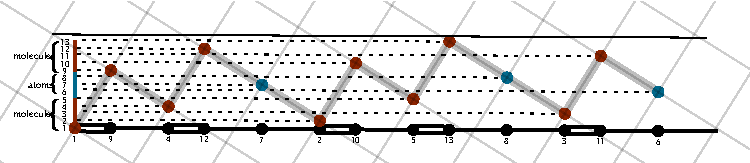
\includegraphics[scale=.9]{img/cut_and_project_perp_projections.pdf}

}
{\flushright
\small{see Mosseri \& Sire 1990.}

}
\(
\<{3cm}
\[
	\id = \frac{j}{L_l}
\]
\>

\<{2cm}
\begin{align*}
	\xleftarrow[]{\text{~~~~conumbering~~~~}} \\
	\xrightarrow[\text{normal numbering}]{}
\end{align*}
\>

\<{3cm}
\[
	\id = \frac{q}{1+\alpha_l} \mod 1
\]
\>
\)
%\begin{tabular}{|c|c|c|}
%\hline 
% & normal numbering & conumbering \\ 
%\hline 
%Atoms & $x_\parallel$ & $x_\perp$ \\ 
%\hline 
%Energy levels & gap label $n$ & normal label $j$ \\ 
%\hline 
%\end{tabular} 

\end{frame}

\begin{frame}{Conumbering and gap labeling}
\(
\<{6cm}
\centering
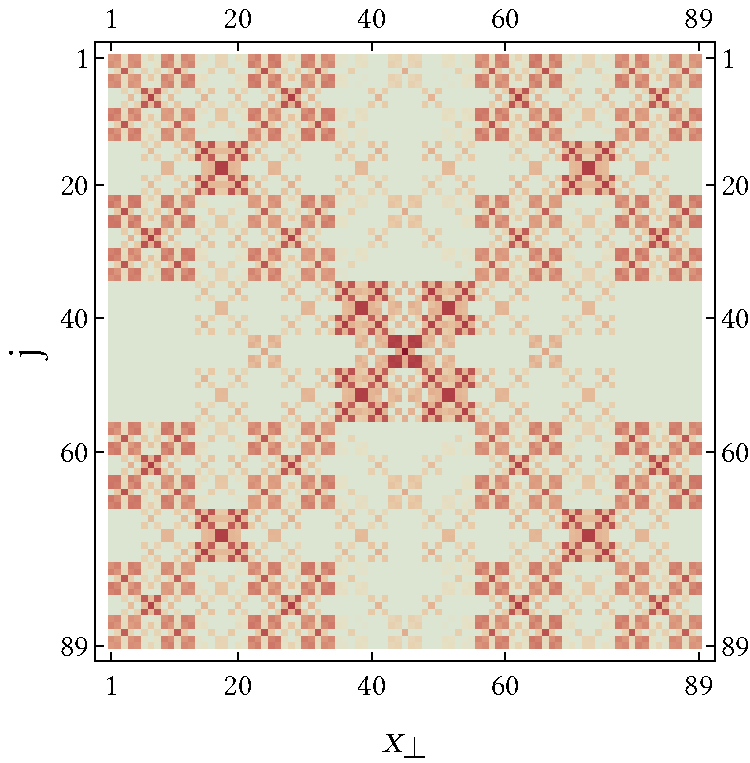
\includegraphics[scale=0.4]{img/ldos_reordered_conumbering.pdf}
\>

\<{6cm}
\centering
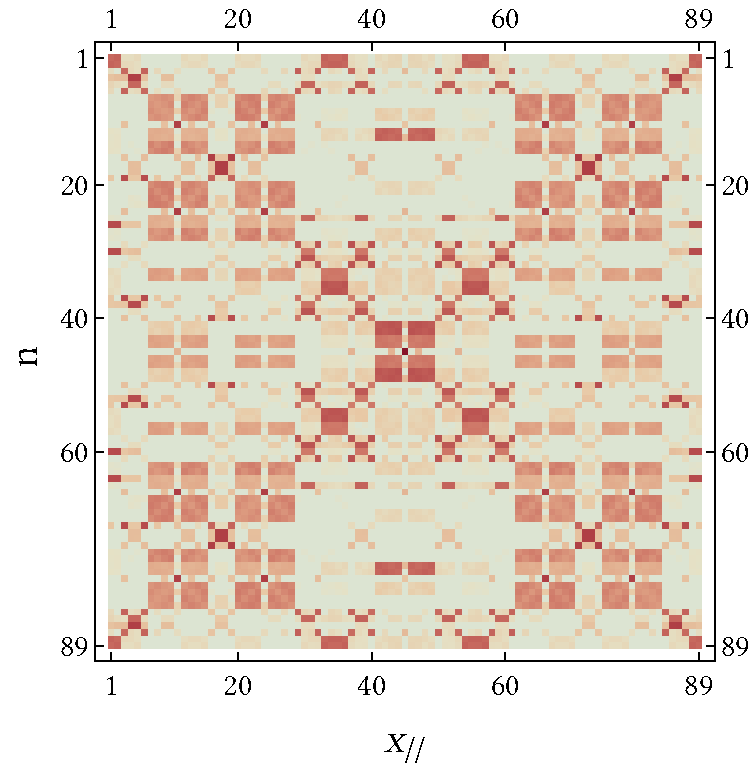
\includegraphics[scale=0.4]{img/ldos_reordered_numbering.pdf}
\>
\)

Plotting the local density of states makes the symmetry between gap labels and atomic labels evident.
\end{frame}

\end{document}
